The handling of systematic uncertainties is separated into normalization uncertainties (those that affect the total yield of a variables' distribution) and shape uncertainties (those that shift the distribution of events). Normalization uncertainties are expressed as multiplicative factors, while shape uncertainties are represented as up and down shifts of a variable's distribution.

Up/down shifts of shape uncertainties can change the number of background events in a distribution. For instance, hadronic taus receive corrections from the nominal tau energy scale, with the nominal, up, and down energy scales provided centrally by CMS. For the $\mu\tau_{h}$ channel, an event could have a $\tau_{h}$ with $p_{T}$ just below the offline threshold of 20 GeV (for instance, 19.5 GeV), so in the nominal distribution of $m_{\tau\tau}$ (or any other variable for this channel), the event is excluded. However, when we build our distributions with the tau energy scale ``up" shift, the energy of this $\tau_{h}$ may be scaled up to, say, 20.5 GeV, and now the event passes the offline $p_{T}$ threshold for the single muon trigger, leading to the event's inclusion in the distributions made with the tau energy scale ``up'' shift.

In evaluating the up and down shifts of a specific source of uncertainty, all other corrections and scale factors are held at their nominal values, and the full chain of object and event selection and event categorization is performed to obtain the observable distributions. Any ``downstream" variables that depend on the shifted variable, e.g. the invariant di-tau mass $m_{\tau\tau}$, must be computed for the nominal case, and then re-computed separately for each up and down shift of the tau legs' energy scale.  The objective of this process is to quantify the effect of a single source of uncertainty on the resulting observable distributions. Each scale factor and correction described in Section \ref{sec:corrections_applied} has an associated uncertainty. The binning of the uncertainties follows that of the nominal scale factor value.

Sections \ref{section:uncertainties_lepton_energy_scales} to \ref{section:MET_uncertainties} describe uncertainties associated with physics objects, and Sections \ref{section:uncertainties_samples} and \ref{section:uncertainties_others} describe uncertainties associated with sample-level effects. The pulls and impacts for the top sixty most important systematics are shown in Section \ref{section:pulls_and_impacts}.



\section{Uncertainties in the lepton energy scales}
\label{section:uncertainties_lepton_energy_scales}
The uncertainties in the tau energy scales~\cite{twiki_TAU_POG_tauidrecommendationforrun2} are binned by the tau decay mode and are taken as shape uncertainties treated as uncorrelated across the tau decay modes and years. Same as with the application of the nominal scale factor, when applying the up or down shifts, the missing transverse energy ($p_{T}^{\text{miss}}$) of the event is adjusted so that the 4-vector sum of the tau $p_{T}^{\text{miss}}$ is unchanged.

The uncertainties in the muon energy scale~\cite{twiki_MUON_POG_recommendation} are 0.4\% for $|\eta| < 1.2$, 0.9\% for $1.2 < |\eta| < 2.1$, and 2.7\% for $2.1 < |\eta| < 2.4$, and are treated as shape uncertainties, fully uncorrelated between embedded and MC samples.

The uncertainties in the electron energy scale~\cite{twiki_Electron_POG_recommendation} in MC are binned in the electron $|\eta|$ and $p_{T}$, and are shown in Fig. \ref{fig:egamma-POG-UL-egamma-scale-factors}. The uncertainties range from 0.5\% to 2.2\% in the barrel, and 0.3\% to 4.1\% in the endcap, across the $p_{T}$ range. The uncertainties for the embedded sample are binned only in $|\eta|$ and are on the order of 0.5\% and 1.25\% for the barrel and endcap~\cite{twiki_embedded_preUL_2018}.

There are also uncertainties in the energy scales for electrons and muons misidentified as $\tau_{h}$. The uncertainty for muons misidentified as $\tau_{h}$ is 1\%~\cite{twiki_TAU_POG_tauidrecommendationforrun2}. For electrons misidentified as $\tau_{h}$, the uncertainty is binned in barrel/endcap $\eta$ and by 1-prong and 1-prong + $\pi_0$ decays. The probability for $e/\mu$ faking a 3-prong decay mode is much lower. 

\section{Uncertainties from other lepton corrections}
Uncertainties associated with the $\tau_{h}$ identification efficiencies are treated as shapes, uncorrelated across the seven $p_{T}$ bins and years. The shape uncertainties in the embedded samples are taken as 50\% correlated with those of the MC samples.

The uncertainties on electron and muon identification efficiencies are taken as normalization uncertainties of 2\% each, with a 50\% correlation between embedded and MC samples.

In the $e\tau_{h}$ channel, there is an additional uncertainty for the vs. jet discrimination efficiency~\cite{twiki_TAU_POG_tauidrecommendationforrun2}, because the analysis uses a looser anti-lepton working point (VLoose WP) than the working points used in the measurement of the efficiency (namely, VLoose WP vs e, and Tight WP vs mu). For nominal $\tau_{h}$ $p_{T} < 100$ GeV, an additional uncertainty of 3\% (5\%) is used in MC (embedded), and for high $p_{T}$ an uncertainty of 15\% is used for both.

The uncertainties in trigger efficiencies are taken as shapes~\cite{twiki_TAU_POG_tauidrecommendationforrun2}. In the $e\tau_{h}$ and $\mu\tau_{h}$ channels, there are uncertainties for the single and cross lepton triggers, and in the $e\mu$ channel there is one uncertainty each for the two $e+\mu$ triggers, and one combined uncertainty since their trigger phase spaces are not mutually exclusive.

\section{Uncertainties from jet energy scale and resolution}
\label{section:JEC_sys}
The jet energy scale uncertainties are taken as shape uncertainties: there are eleven in total, with seven correlated across years (labeled ``Year" below) and the remainder uncorrelated across years. They affect the b-tag jet $p_{T}$ and mass, and hence the missing transverse energy $p_{T}^{\text{miss}}$. The shifts are propagated through the b-tagging scale factor calculation and b-tag jet counting. 

The uncertainties in the jet energy correction and resolution~\cite{CMS-JME-13-004}~\cite{twiki_JetEnergyScale_Uncertainty_Sources_JERC} are as follows:
    \begin{itemize}
        \item \textit{Absolute, AbsoluteYear}: flat absolute scale uncertainties.
        \item \textit{BBEC1, BBEC1Year}: for sub-detector regions, with barrel ``BB" in $|\eta| < 1.3$ and endcap region 1 ``EC1'': $1.3 < |\eta| < 2.5$.
        \item \textit{EC2, EC2 year}: for sub-detector regions, with endcap region 2 ``EC2'' in $2.5 < |\eta| < 3.0$.
        \item \textit{HF, HF year}: for sub-detector regions, with hadron forward ``HF'' in $|\eta| > 3$.
        \item \textit{FlavorQCD}: for uncertainty in jet flavor (uds/c/b-quark and gluon) estimates based on comparing Pythia and Herwig (different MC generator) predictions. 
        \item \textit{RelativeBal}: account for difference between log-linear fits of the two methods used to study the jet energy response: MPF (missing transverse momentum projection fraction) and $p_{T}$ balance.
        \item \textit{RelativeSample}: account for $\eta$-dependent uncertainty due to a difference between relative residuals, observed with dijet and Z+jets in Run D of 2018 data.
        \item \textit{JetResolution}: uncertainty in the jet energy resolution.
    \end{itemize}

\section{Uncertainties from b-tagging scale factors}
The b-tagging scale factor has its own set of associated uncertainties (not to be confused with shifts in the b-tagging scale factor due to the propagation of the jet energy scale uncertainties described in the previous section \ref{section:JEC_sys}). They are:
\begin{itemize}
    \item \textit{hf}: contamination from heavy flavor (b+c) jets in the light flavor region.
    \item \textit{hfstats1, hfstats2}: linear and quadratic statistical fluctuations from b-flavor jets. 
    \item \textit{lf}: contamination from light flavor (udsg+c jets) in the heavy flavor region.
    \item \textit{lfstats1, lfstats2}: linear and quadratic statistical fluctuations from udsg jets.
    \item \textit{cferr, cferr2}: uncertainty for charm jets.
\end{itemize}
The variations for ``lf, hf, hfstats1/2, lfstats1/2'' are applied to both b and udsg jets. For c-flavor jets, only ``cferr1/2'' is applied.

\section{Uncertainties from MET}
\label{section:MET_uncertainties}
Samples where recoil corrections were applied (Z+jets, W+jets, and Standard Model Higgs, as described in Section \ref{sec:corrections_applied}) have uncertainties from the response and resolution of the hadronic recoil against the leptonic system. These are each binned in jet multiplicity.

\section{Uncertainties associated with samples used}
\label{section:uncertainties_samples}
Normalization uncertainties related to the samples used are:
\begin{itemize}
    \item \textit{Cross-section uncertainties}: $\sigma(t\bar{t})$: 4.2\%, $\sigma$(diboson): 5\%,  $\sigma$(single top): 5\%, $\sigma$(ggH): 3.2\%, $\sigma$(qqH): 2.1\%, $\sigma$(WH): 1.9\%, $\sigma$(ZH): 1.3\%, $\sigma$(ttH): 3.6\%
    \item \textit{Uncertainties in QCD renormalization scale}: QCD scale(qqH): +0.43\%-0.33\%, QCD scale(WH): +0.5\%-0.7\%, QCD scale(ttH): +5.8\%-9.2\%
    \item \textit{Branching ratio uncertainties}: BR(H$\rightarrow\tau\tau$): 1.8\%, and BR(H$\rightarrow$WW): 1.5\%.
    \item \textit{Normalization uncertainties}: 2\% for Drell-Yan, 4\$ for embedded, 20\% pre-fit for the QCD multijet background in the $e\mu$ channel, 20\% pre-fit for the jet faking background.
\end{itemize}

The $t\bar{t}$ process has additional acceptance uncertainties from QCD scale variation and parton shower uncertainties~\cite{twiki_Top_systematics}.  Parton shower uncertainties originate from the modeling of perturbative and non-perturbative QCD effects handled in parton shower MC generators. The scale variations are determined from the envelope of the 6 provided shapes due to variations in the factorization scale, renormalization scale, and their combined variation~\cite{twiki_Top_systematics}.

The Z $p_{T}$ reweighing uncertainty in Drell-Yan samples is taken to be 10\% of the nominal value, taken as a shape uncertainty. 

The fake rate uncertainties are taken as shape uncertainties. For the weight applied to scale up anti-isolated events in cross-trigger regions, 20\% of the nominal weight is taken as a shape uncertainty.

\section{Other uncertainties}
\label{section:uncertainties_others}
A 3.6\% yield uncertainty in the signal is used to cover uncertainties in the parton distribution functions, $\alpha_s$ (fine structure constant), and QCD scale. 

Normalization uncertainties from luminosity are applied to all MC samples, divided into those uncorrelated across years, those correlated between 2017 and 2018, and one for 2018~\cite{twiki_LUMI_POG_recommendation}.

\section{Pulls and impacts}
\label{section:pulls_and_impacts}
The top impacts and pulls computed for the combination of all channels and years is shown in Fig. \ref{fig:impacts_pages_1_2}. The top impacts are related to uncertainty in the signal sample and cross-section of the $t\bar{t}$ cross-section, and also the yields of the jet faking $\tau_{h}$ background, which is a major background in all channels and expected to be constrained due to the yield uncertainty which is taken to be 20\% pre-fit. 

\begin{figure}[ht]
    \begin{center}
        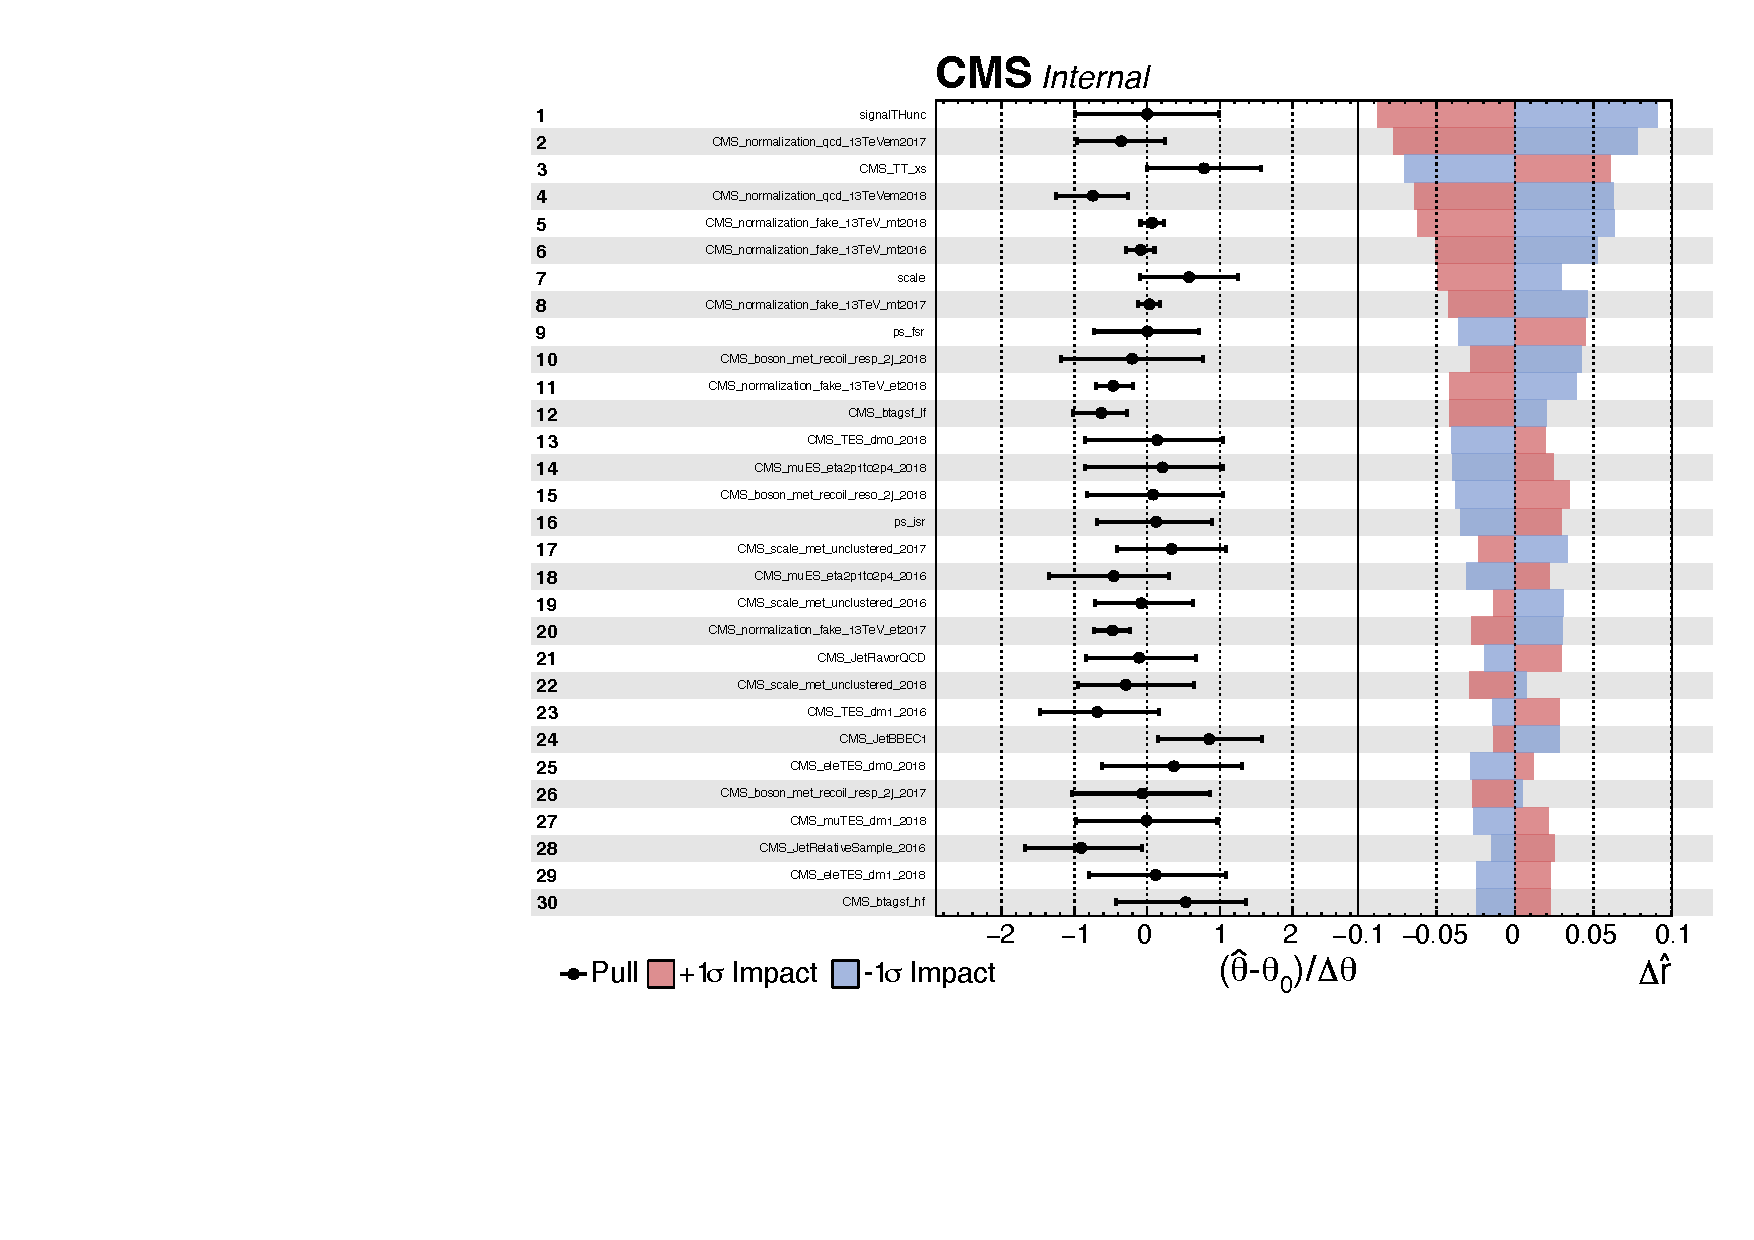
\includegraphics[width=0.8\textwidth]{figures/ch-8-systematic-uncertainties/impacts-all-1.pdf}\\
        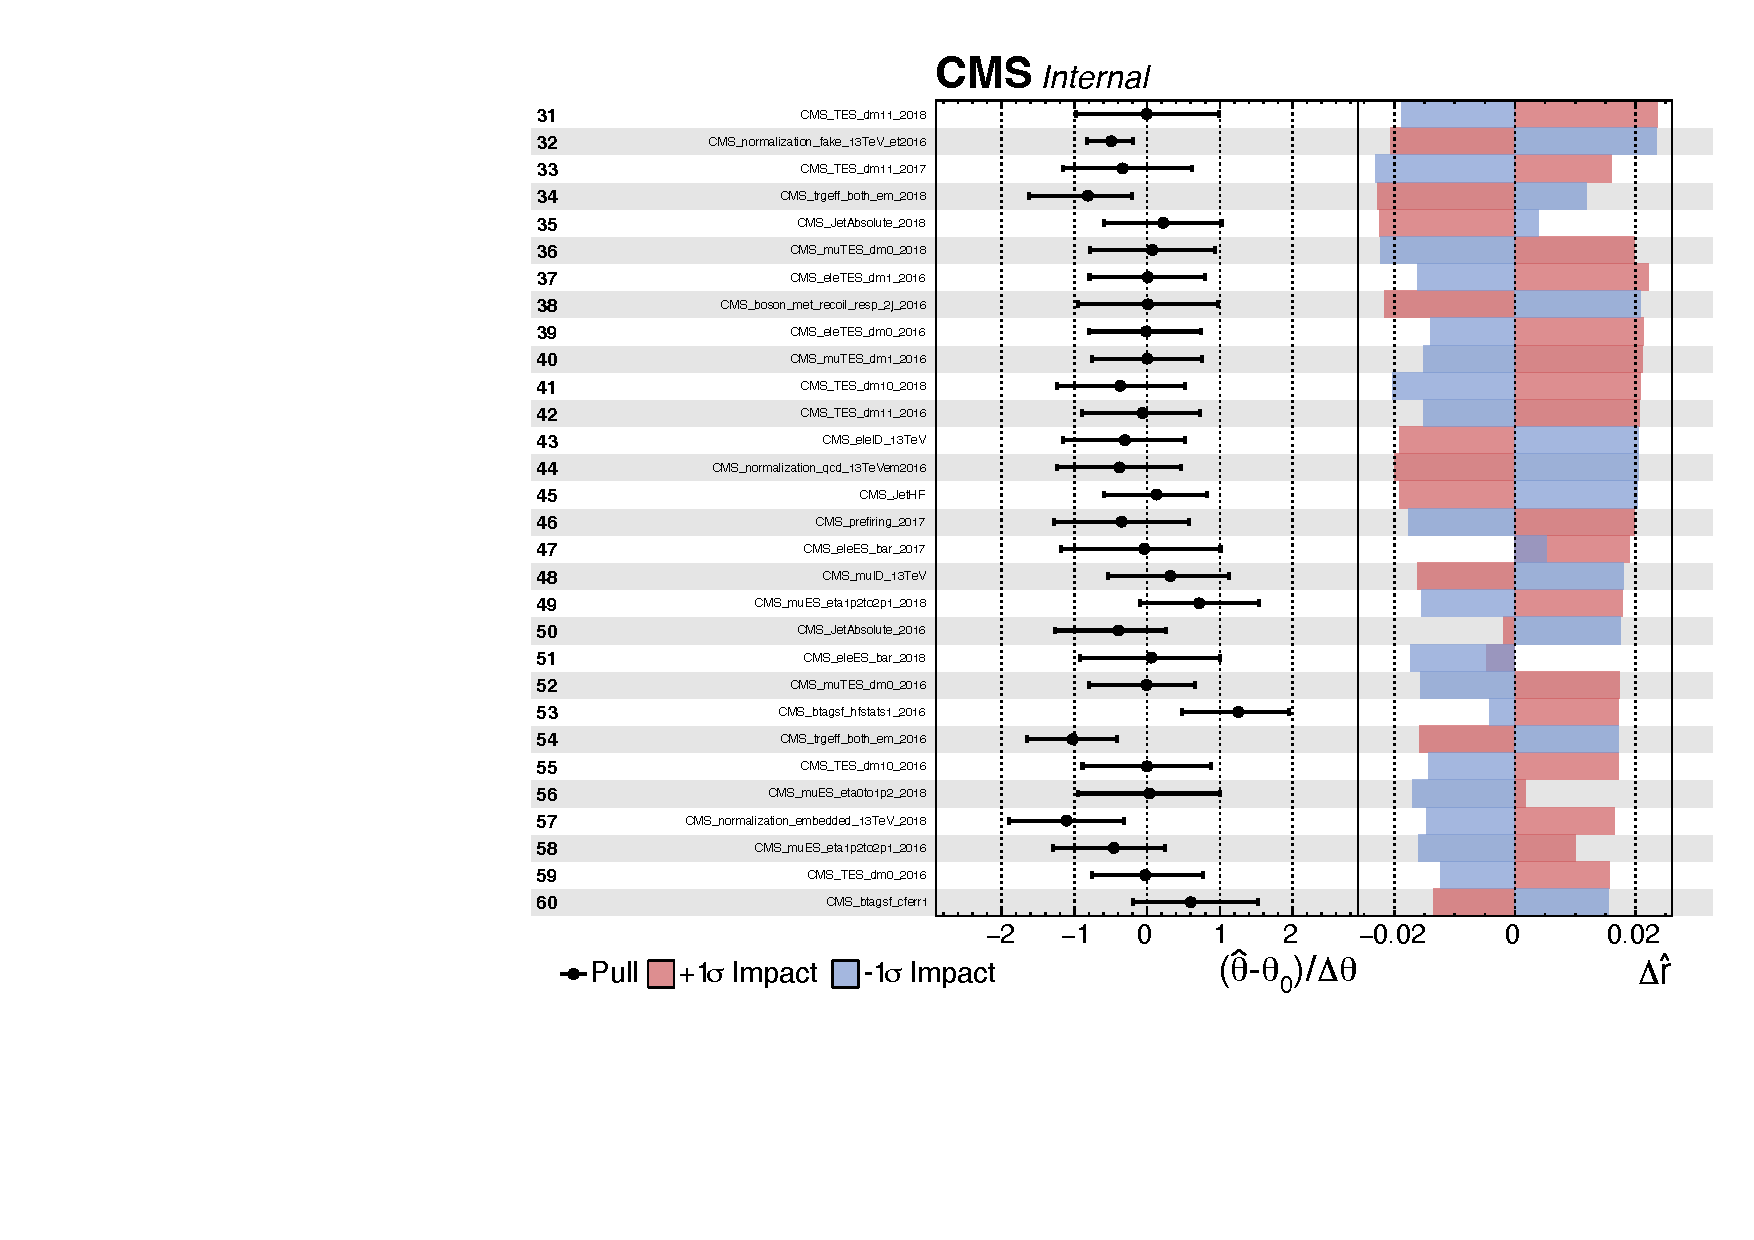
\includegraphics[width=0.8\textwidth]{figures/ch-8-systematic-uncertainties/impacts-all-2.pdf}
    \end{center}
    \caption[Top sixty pulls and impacts for the combination of all channels and years.]{Top sixty pulls and impacts for the combination of all channels and years~\cite{CMS-AN-20-213}.}
    \label{fig:impacts_pages_1_2}
\end{figure}
